%% Bench 2026 / PEvaluation submission version (anonymized).
%% Adapted from artigo/main.tex (SBC format, Portuguese) to TBench-template.
%% Content preserved; translated to academic English; double-blind anonymized.
\documentclass[namedate,webpdf,contemporary,large]{TBench-template}%
\usepackage[english]{babel}
\usepackage{booktabs}
\usepackage{adjustbox}
\usepackage{graphicx}
\usepackage{xcolor}
\usepackage{tikz}
\usepackage{pgfplots}
\usepgfplotslibrary{groupplots}
\usetikzlibrary{arrows.meta,positioning}
\pgfplotsset{compat=1.18, table/col sep=comma}
\makeatletter
\AtBeginDocument{
    \renewcommand*{\citenumfont}{\color{jnlclr}}
}
\makeatother

\theoremstyle{thmstyleone}%
\newtheorem{theorem}{Theorem}%
\newtheorem{proposition}[theorem]{Proposition}%
\theoremstyle{thmstyletwo}%
\newtheorem{example}{Example}%
\newtheorem{remark}{Remark}%
\theoremstyle{thmstylethree}%
\newtheorem{definition}{Definition}

\begin{document}

\journaltitle{BenchCouncil Transactions on Benchmarks, Standards and Evaluations}
\DOI{DOI HERE}
\copyrightyear{2026}
\pubyear{2026}
\appnotes{Original Article}

\firstpage{1}

\title[Symmetric Preprocessing for Sorting Algorithms]{Impact of $O(n)$ Symmetric Preprocessing on Inversion Reduction and Sorting Algorithm Efficiency: An Experimental Evaluation Across Adaptive and Non-Adaptive Methods}

% Anonymized for double-blind review: no author, address, or corresp info included.

\received{Date}{0}{Year}
%\revised{Date}{0}{Year}
\accepted{Date}{0}{Year}

\abstract{Quadratic sorting algorithms remain relevant in resource-constrained systems but are sensitive to inversion counts. This study investigates the impact of inversions on sorting performance and their reduction through preprocessing. The objective is to assess the effectiveness of this technique for adaptive and non-adaptive algorithms. Five algorithms were compared across six input topologies, using vectors of up to $10^5$ elements for quadratic methods and $10^6$ for quasilinear methods with $O(n)$ preprocessing. The technique reduced inversions by 40--62\% on non-aligned inputs at about 1.2 ns per element, with extreme reductions (99.99--100\%) restricted to inputs geometrically aligned with the symmetric scan (Reversed, Zigzag). On non-aligned inputs, adaptive quadratic methods gained 13--42\% (speedups up to $\times$2,073 on aligned inputs), while the evaluated $O(n \log n)$ implementations showed mixed results for Merge Sort and systematic degradation for Quicksort.}
\keywords{Sorting algorithms, Adaptive sorting, Presorting, Benchmarking, Performance evaluation, Experimental methodology}

\maketitle

\section{Introduction}\label{sec:intro}
Sorting is a fundamental operation in computer science, essential in search systems, databases, and real-time applications \cite{knuth_art_1973,sedgewick_algorithms_2011}. Although methods with $O(n \log n)$ asymptotic complexity, such as Merge Sort and Quicksort, are preferable for large data volumes, quadratic $O(n^2)$ algorithms such as Insertion Sort, Selection Sort, and Bubble Sort remain relevant in specific scenarios \cite{cormen_introduction_2022}. This persistence relates to structural simplicity, low memory consumption through in-place operation, and practical efficiency on small or partially ordered datasets \cite{cormen_introduction_2022,ziviani_projeto_2021}.

The practical efficiency of a sorting algorithm does not depend exclusively on its asymptotic complexity; it is also influenced by properties of the input sequence \cite{estivill-castro_survey_1992}. In this context, an inversion, defined as a pair satisfying $A[i] > A[j]$ for $i < j$, constitutes a quantitative measure of the disorder degree of an array \cite{knuth_art_1973,mannila_measures_1984}. The inversion count characterizes different levels of presortedness, since sequences with more inversions exhibit greater disorder relative to the final order \cite{mannila_measures_1984}. This characteristic can significantly influence execution cost, especially for algorithms whose operation count depends on input disorder \cite{estivill-castro_survey_1992}.

Despite this relation between input disorder and execution cost, quadratic algorithms may exhibit limited adaptability to initial data conditions \cite{mannila_measures_1984,estivill-castro_survey_1992}. In particular, inputs with many inversions can increase required movements during sorting, degrading performance of methods such as Insertion Sort \cite{cormen_introduction_2022}. In this scenario, a preliminary step capable of reducing input disorder may decrease the subsequent work of the sorting algorithm. The research question is therefore: to what extent does a preprocessing step aimed at inversion reduction impact the practical performance of quadratic and quasilinear sorting algorithms?

Formally, let $C_{\text{original}}$ denote the temporal cost of directly sorting the input. By introducing symmetric preprocessing with cost $C_{\text{pre}}$, the subsequent sorting algorithm operates on a modified vector, spending a reduced time $C_{\text{sort}}$. The objective of this work is to propose, implement, and evaluate a low-cost $O(n)$ symmetric preprocessing algorithm designed to reduce the inversion count of an input vector. We empirically verify whether the hybrid approach is more time-efficient than directly applying the same conventional algorithm, identifying the practical conditions under which $C_{\text{pre}} + C_{\text{sort}} < C_{\text{original}}$ holds. Comparison against the fastest available general sorter (rather than the same algorithm) and a formal closed-form theory of expected reduction are left as future work.

The relevance of this study lies in investigating a strategy capable of improving practical sorting behavior without modifying fundamental structure or introducing high additional cost. Reducing disorder before the main sort may decrease operations on unfavorable inputs, especially in methods sensitive to inversion counts \cite{estivill-castro_survey_1992,hwang_presorting_2000}. The study also contributes to adaptive-algorithm analysis by investigating conditions under which preprocessing cost is compensated by reduced sorting work \cite{mannila_measures_1984,hwang_presorting_2000}.

The research adopts a quantitative, applied, and experimental approach \cite{gil_metodos_2019,sampieri_metodologia_2021}. The study comprises formal modeling of the preprocessing algorithm and its implementation in Rust. Experimental evaluation used automated benchmarks with the Criterion library, employing synthetic vectors ranging from 1,000 to 1,000,000 elements with controlled inversion levels, covering worst cases, partial ordering, and adversarial structured topologies inspired by classical sorting-test patterns. Experiments compared execution time of the hybrid approach against directly applied sorting algorithms on the same inputs.

This article is structured as follows. Section~\ref{sec:background} presents theoretical background. Section~\ref{sec:method} describes methodology, formalization of the proposed preprocessing algorithm, evaluated sorting algorithms, and experimental procedures. Section~\ref{sec:results} presents and discusses results. Finally, Section~\ref{sec:conclusion} presents conclusions.

\section{Background and Related Work}\label{sec:background}
This section presents the theoretical foundations: inversions as a disorder measure, adaptive-sorting principles, characteristics of evaluated algorithms including quadratic and quasilinear methods, preprocessing concepts and symmetric-preprocessing principles, and related work situating this contribution.

\subsection{Inversions and Adaptive Sorting}
Practical efficiency of traditional sorting algorithms often depends on initial element disposition \cite{cormen_introduction_2022,estivill-castro_survey_1992}. To formalize the disorder degree, the classical concept of \emph{inversion} is used \cite{knuth_art_1973}. Given a vector $a$ of $n$ elements, an inversion is formally a pair $(i,j)$ such that $i < j$ and $a[i] > a[j]$ \cite{knuth_art_1973,sedgewick_algorithms_2011}. The total inversion count $I$ measures input disorder and relates directly to effort required to sort via local operations \cite{mannila_measures_1984}.

The relation between inversion volume $I$ and execution complexity gives rise to \emph{adaptivity} \cite{estivill-castro_survey_1992}. An algorithm is adaptive when its time complexity improves markedly in the presence of partial presortedness \cite{mannila_measures_1984}. A classical example is \emph{Insertion Sort}, consuming $O(n+I)$ operations. On a strictly ordered vector ($I=0$) it reaches linear $O(n)$ time, while in the worst case ($I=O(n^2)$) it degrades to quadratic time \cite{cormen_introduction_2022,knuth_art_1973}.

\subsection{Evaluated Algorithms}
To evaluate symmetric-preprocessing impact across sorting paradigms, a representative set with distinct time complexity, adaptivity, and sensitivity to initial order was selected, covering both methods whose efficiency may be directly influenced by disorder and methods less dependent on it.

In the quadratic $O(n^2)$ worst-case group, \emph{Bubble Sort}, \emph{Insertion Sort}, and \emph{Selection Sort} were evaluated \cite{cormen_introduction_2022}. \emph{Insertion Sort} is adaptive in the inversion count ($O(n+I)$); \emph{Bubble Sort} with early exit is adaptive in the number of passes---which is governed by the maximum left-displacement of any element rather than by the total $I$---while \emph{Selection Sort} is non-adaptive and maintains fixed comparisons regardless of initial configuration \cite{estivill-castro_survey_1992}. This distinction matters for interpreting results: inversion elimination translates directly into fewer shifts for Insertion Sort, whereas Bubble Sort gains arise only when preprocessing collapses the maximum displacement (as in Zigzag and Reversed inputs).

In the quasilinear group, \emph{Merge Sort} with $O(n \log n)$ time and \emph{Quicksort} with $O(n \log n)$ average performance (though $O(n^2)$ worst case) were evaluated \cite{cormen_introduction_2022}. Their inclusion verifies whether effects observed in quadratic algorithms remain relevant at lower asymptotic cost, extending analysis beyond inversion-count-related algorithms.

Thus the set covers three relevant dimensions: adaptive quadratic algorithms (\emph{Bubble Sort} and \emph{Insertion Sort}), a non-adaptive quadratic algorithm (\emph{Selection Sort}), and quasilinear algorithms based on distinct strategies (\emph{Merge Sort} and \emph{Quicksort}). This composition verifies not only whether symmetric preprocessing reduces inversions, but to what extent this reduction converts into gains for algorithms with different dependence on initial order.

\subsection{Symmetric Preprocessing Concept}
Preprocessing, in algorithm design and analysis, refers to a preliminary transformation of input data before the main algorithm \cite{cormen_introduction_2022}. Its purpose is to alter instance disposition, making subsequent resolution simpler or more efficient. Conceptually, preprocessing acts analogously to prior organization of a work environment: although preparation requires initial cost, reduced main-processing effort compensates it.

For viability in sorting, preprocessing temporal cost must be strictly dominated by the succeeding sorting complexity \cite{cormen_introduction_2022,sedgewick_algorithms_2011}. An ideal preprocessing should exhibit linear $O(n)$ time, ensuring overhead is asymptotically negligible relative to total sorting cost---whether $O(n \log n)$ average quasilinear or $O(n^2)$ worst-case quadratic \cite{knuth_art_1973}.

In this research, preprocessing is termed \emph{symmetric} because it applies a bidirectional mirrored scan from vector ends. This restructuring aims to reduce total inversions $I$ by moving discrepant elements closer to final destinations in a single $O(n)$ pass. By providing a partially reordered structure, it seeks to mitigate comparisons and swaps in both adaptive and non-adaptive methods.

\subsection{Related Work}
Literature presents different approaches to characterize sequence sortedness and exploit it. Mannila \cite{mannila_measures_1984} studied presortedness and established measures quantifying disorder forms. The author defined general properties for presortedness measures and introduced optimal sorting relative to a measure. Among measures is inversion count $Inv(X)$. The work presented optimal algorithms for different measures and showed \emph{Insertion Sort} optimal for three natural measures, establishing foundations for adaptive algorithms~\cite{mannila_measures_1984}.

Estivill-Castro and Wood \cite{estivill-castro_survey_1992} surveyed adaptive sorting, considering input disorder degree. The work presented main concepts, disorder measures, and established results on \emph{adaptive sorting}, synthesizing theoretical and practical results including relations between disorder measures and algorithms exploiting presortedness. The survey records that several algorithms exhibit complexity dependent on both input size and disorder, and that certain adaptive algorithms perform competitively on random sequences with significant gains on nearly sorted inputs.

In an approach directly related to preliminary transformations, Hwang, Yang, and Yeh \cite{hwang_presorting_2000} investigated \emph{presorting} algorithms from an average-case perspective, using inversion-count reduction as performance measure. The authors formulated quantification of preliminary-step effects via average inversion reduction, analyzing steps of known algorithms including \emph{Shellsort} and \emph{Quicksort}, and derived expectation, variance, and generating functions of that reduction. Their framework could in principle host a closed-form derivation of the expected reduction of symmetric preprocessing under uniform random input; such a derivation is left as future work. Empirically, the average reduction on random input was $\sim$45\% of the initial $\Theta(n^2)$ inversions (Table~\ref{tab:inversions})---a large absolute $\Theta(n^2)$ reduction produced by a linear pass, whose precise expectation requires the generating-function machinery of \cite{hwang_presorting_2000}.

Recent literature reinforces practical relevance of microarchitectural effects. Edelkamp and Weiss~\cite{edelkamp_blockquicksort_2016} showed branch mispredictions can dominate Quicksort cost and proposed \emph{BlockQuicksort}, providing basis for degradation hypotheses for \emph{Selection Sort} and Quicksort in this work. Auger et al.~\cite{auger_timsort_2018} analyzed \emph{Timsort} worst-case complexity, showing exploitation of pre-existing runs remains an active sorting-engineering theme. LaMarca and Ladner~\cite{lamarca_influence_1999} showed cache influence on sorting performance, also discussed by Kaligosi and Sanders~\cite{kaligosi_branch_2006} when quantifying branch-misprediction impact. These works position the present low-cost technique as a preprocessing-heuristic instance whose trade-off must be jointly evaluated at logical (inversions) and microarchitectural levels.

Differing from mapped approaches, this research evaluates a Symmetric Preprocessing algorithm acting on direct inversion mitigation in linear time, as one low-cost preprocessing instance. A systematic comparison against Shell-type passes and run-detection heuristics, and a formal gap analysis, remain future work.

\section{Experimental Methodology}\label{sec:method}
This work follows an applied, quantitative, experimental evaluation design \cite{gil_metodos_2019,sampieri_metodologia_2021}: it controllably manipulates input topology and size (independent variables) and observes execution time and inversion counts (dependent variables) under a fixed seed, paired vector generation, and a standardized environment. From an evaluation-methodology standpoint, the study is framed as a cost--benefit assessment of a preprocessing pass: the measured total $C_{\text{pre}}+C_{\text{sort}}$ internalizes preprocessing overhead, the paired design controls input variability as a confounder, and correctness is checked outside the timed region. Three working hypotheses guide the analysis: (H1) adaptive quadratic algorithms benefit where absolute inversion reduction $\Delta I$ is large; (H2) the non-adaptive quadratic algorithm is neutral to inversion reduction; (H3) for quasilinear methods the overhead $C_{\text{pre}}$ dominates unless structural disorder is extreme.

\subsection{Experimental Configuration}
Experiments ran in a controlled environment whose hardware, OS, and tool specifications appear in Table~\ref{tab:environment}. To reduce variability, power plan was kept at high performance and background processes minimized. Code was compiled in \emph{release} mode with maximum optimization (\texttt{opt-level = 3}). Input generation used a fixed seed, ensuring reproducibility and correspondence across experimental conditions.

% Tabela 1

\begin{table}[!t]
\caption{Experimental environment and tools.\label{tab:environment}}%
\begin{tabular*}{\columnwidth}{@{\extracolsep\fill}ll@{\extracolsep\fill}}
\toprule
Component & Configuration / Specification\\
\midrule
Operating system & Windows 11 Pro (build 10.0.26200)\\
Processor & AMD Ryzen 7 8700G\\
Memory & 16 GB DDR5 5600MT/s\\
Language & Rust 1.96.0 (release profile)\\
Measurement tools & Criterion 0.5 and Project CLI Tool\\
Data generation & Seed 42 (\texttt{ChaCha8Rng}), paired inputs\\
\botrule
\end{tabular*}
\end{table}

To evaluate resilience under different entropy degrees, six structural input patterns were implemented with the exact generators in Table~\ref{tab:datasets} (0-based indices, values in \texttt{i32}). For each topology-size combination, a single pool of 50 vectors is generated with \texttt{ChaCha8Rng} seeded by $42 \oplus n \oplus \text{type}$ and shared by all algorithms and both variants (pure and preprocessed), ensuring paired comparability. Deterministic generators (Reversed, Zigzag, Turtles) yield identical vectors across the 50 pool slots; stochastic generators (Random, Duplicates, Almost Sorted) advance the same RNG stream, so slot $k$ differs across slots but is identical across algorithms and variants for fixed $k$.

Quasilinear algorithms (\emph{Merge Sort} and \emph{Quicksort}) were measured at $n \in \{1{,}000, 5{,}000, 10{,}000, 100{,}000, 1{,}000{,}000\}$. For quadratic algorithms (\emph{Insertion Sort}, \emph{Bubble Sort}, \emph{Selection Sort}), measurements were restricted to $n \le 100{,}000$: at $n=10^6$ each execution would take minutes, precluding systematic collection of statistically significant samples. This restriction is documented and does not compromise comparison, as gain orders of magnitude already stabilize at $n=100{,}000$.

Isolated preprocessing cost ($C_{\text{pre}}$) was additionally characterized at $n \in \{1{,}000, 5{,}000, 10{,}000, 20{,}000, 100{,}000, 1{,}000{,}000\}$ (Table~\ref{tab:precost} and Fig.~\ref{fig:precost}) to evidence linearity; the $n{=}20{,}000$ point was collected exclusively for this cost curve via CLI tool (\texttt{seed} 42), under the same paired-generation protocol, and is not part of the main sorting-time comparison matrix.

% Tabela 2

\begin{table}[!t]
\caption{Input-topology generators ($n$ = size, 0-based index $i$).\label{tab:datasets}}%
\begin{tabular*}{\columnwidth}{@{\extracolsep\fill}ll@{\extracolsep\fill}}
\toprule
Topology & Exact Generator\\
\midrule
Random & \texttt{shuffle} of $[0,n{-}1]$ with \texttt{ChaCha8Rng}\\
Turtles & $a[i]=i+n$ if $i<n/2$, else $a[i]=i \bmod 10$\\
Zigzag & $a[i]=i$ if $i$ even, else $a[i]=n-i$\\
Almost Sorted & $[0,n{-}1]$ with $n/100$ uniform pair swaps $(i,j)$, $i\neq j$\\
Duplicates & $a[i]\sim\mathcal{U}\{0,1,2\}$ i.i.d.\\
Reversed & $a[i]=n-i$ (strictly decreasing)\\
\botrule
\end{tabular*}
\end{table}

\subsection{Evaluated Algorithm Specifications}
To ensure internal validity, timing stability, and reproducibility, all sorting algorithms were implemented in Rust (version 1.96.0), operating directly on mutable slices of 32-bit integers (\texttt{\&mut [i32]}). Implementations avoided high-level external abstractions, standardizing memory handling and adopting idiomatic instruction-level optimizations.

\subsubsection{Quadratic Algorithms}
\begin{itemize}
\item \textbf{Bubble Sort:} Optimized adaptive version. Successive scans reduce upper bound each iteration ($n-1-i$). Adaptivity is ensured by a boolean flag (\texttt{swapped}) monitoring swaps per pass; if a scan completes with no element permutation, execution halts early, ensuring $O(n)$ on presorted vectors.
\item \textbf{Insertion Sort:} Traditional direct-insertion by shifting. For each element of the unordered sub-slice, current value is stored in a temporary variable and strictly greater antecedents are shifted right. Search and shifting end once correct position is found or left bound ($j=0$) is reached, minimizing write overhead versus successive-swap implementations.
\item \textbf{Selection Sort:} Classical non-adaptive in-place form. At each outer iteration $i$, the algorithm scans unordered segment $[i+1,n-1]$ to identify minimum-element index. Swap with position $i$ executes conditionally only if minimum resides at a distinct index. Comparison cost remains strict $O(n^2)$, regardless of presortedness.
\end{itemize}

\subsubsection{Quasilinear Algorithms}
\begin{itemize}
\item \textbf{Merge Sort:} Top-down divide-and-conquer with stable ordering guarantee. To eliminate continuous dynamic-allocation overhead distorting timings, implementation allocates a single temporary auxiliary vector of size $n$ at function entry, passed by mutable reference through recursive calls. Sub-slice midpoints use right bit-shifting ($(\text{end}-\text{start}) \gg 1$), avoiding integer division. Merge copies current-slice data to auxiliary buffer and rebuilds ordered segment with three index pointers.
\item \textbf{Quicksort:} Recursive implementation using three-way partitioning (\emph{Dutch National Flag} / Dijkstra's algorithm) with median-of-three pivot selection. Pivot is median among initial, central, and final subvector elements. Three-way partitioning rearranges into three contiguous regions: less than, equal to, and greater than pivot, maintaining \texttt{lt}, \texttt{i}, \texttt{gt} indices. This yields $O(n \log n)$ average time and robustness to many duplicate keys (no worst-case guarantee: median-of-three does not preclude $O(n^2)$ on adversarial inputs). Tail-call optimization iterates on the larger partition and recurses on the smaller.
\end{itemize}
In all implementations, preliminary boundary checks (\emph{early returns}) ensure slices with $n<2$ return immediately without function calls or unnecessary allocations.

\subsection{Experimental Protocol and Inversion Counting}
Empirical measurement used the \emph{Criterion.rs} framework: warm-up cycles mitigate cache effects, and bootstrap resampling estimates 95\% confidence intervals (\texttt{confidence\_level=0.95}, \texttt{significance\_level=0.05}). Each Criterion sample clones the next pool vector in rotation (\texttt{iter\_batched}, per-iteration \texttt{clone} outside the timed region), so the 50-vector pool feeds all samples while cloning cost is never timed; only $C_{\text{total}} = C_{\text{pre}} + C_{\text{sort}}$ is timed in the preprocessed variant.

Measurement configuration was profile-adjusted (configured values; Criterion may extend effective measurement to reach statistical stability): 50 samples with 2\,s warm-up and 5\,s measurement window for most scenarios; for quadratic algorithms at $n=100{,}000$ (iterations up to $\approx$2\,s for Selection Sort), 30 samples with 1\,s warm-up and 5\,s window; and for quasilinear methods at $n=10^6$, 50 samples with 2\,s warm-up and 10\,s window. Mean, median, and 95\% CIs are computed per cell; tables report mean $\pm$ CI half-width.

Statistical criterion: a variation was considered relevant when 95\% confidence intervals of the two conditions (pure vs.\ preprocessed) do not overlap. When CIs overlap, variation was treated as non-significant regardless of point percentage difference. This criterion is exploratory and conservative (the design is paired, but the analysis treats cells as independent); it was uniformly applied throughout Section~\ref{sec:results} to qualify expressions such as ``consistent gain,'' ``systematic degradation,'' and ``mixed results.'' A paired bootstrap analysis of per-vector time ratios remains future work.

Beyond timing, correctness of each scenario was verified outside the timed region: for every (algorithm, topology, size), the sorted output is checked element-wise ($a[0]\le a[1]\le\cdots$) and against \texttt{sort\_unstable} in both pure and preprocessed variants. Inversion counts of each shared-pool vector, before and after preprocessing, are recorded in harness companion files, ensuring inversion tables derive from exactly the same timed vectors.

Exact inversion-count quantification uses a modified-MergeSort-based $O(n \log n)$ implementation \cite{cormen_introduction_2022}. During merging of two ordered subvectors $L$ and $R$, when $R[j]$ is less than $L[i]$, exactly $|L|-i$ is added to the counter. This eliminates $O(n^2)$ direct-counting bottleneck, enabling evaluation of $10^5$--$10^6$-element vectors.

\subsection{Symmetric Preprocessing Formalization}
The proposed symmetric preprocessing operates as a deterministic single-pass scan over input vector $A$ of size $n$. Its goal is restructuring via mirrored swaps and local adjustments before evaluated sorting algorithms. Procedural structure is formalized in Algorithm~\ref{alg:preproc}.

% Algoritmo

\begin{algorithm}[!t]
\caption{Symmetric Preprocessing Algorithm}\label{alg:preproc}
\begin{algorithmic}[1]
\Require Vector $A$ of size $n$
\Ensure Partially reorganized vector $A$
\State $n \gets$ size of $A$
\If{$n < 2$}
\State \Return
\EndIf
\State $last \gets n-1$
\State $mid \gets \lfloor n/2 \rfloor$
\For{$i \gets 0$ \textbf{to} $mid-1$}
\State $j \gets last-i$
\If{$A[i] > A[j]$}
\State swap($A[i], A[j]$)
\EndIf
\If{$i+1 < mid$}
\If{$A[i] > A[i+1]$}
\State swap($A[i], A[i+1]$)
\EndIf
\EndIf
\If{$j-1 > mid$}
\If{$A[j] < A[j-1]$}
\State swap($A[j], A[j-1]$)
\EndIf
\EndIf
\EndFor
\end{algorithmic}
\end{algorithm}

The algorithm iterates over the first half, scanning $i \in [0, \lfloor n/2 \rfloor - 1]$. Each iteration computes the symmetric index at the opposite end, $j=(n-1)-i$. Loop execution comprises three structured conditionals: (1) \textbf{Extreme symmetric swap:} if $A[i] > A[j]$, direct swap places smaller element in left segment and larger in right; (2) \textbf{Left adjacent adjustment:} for $(i+1) < \lfloor n/2 \rfloor$, if $A[i] > A[i+1]$, swap adjacent elements; (3) \textbf{Right adjacent adjustment:} for $(j-1) > \lfloor n/2 \rfloor$, if $A[j] < A[j-1]$, swap adjacent elements.

Boundary conditions ensure adjacent swaps operate strictly within respective subdomains without crossing the midpoint: the left adjustment covers pairs up to $(mid{-}2,mid{-}1)$ and the right adjustment from $(mid{+}1,mid{+}2)$ onward, so neither side touches a midpoint-crossing adjacent pair and the procedure is left-right symmetric. Computationally, the algorithm executes exactly $\lfloor n/2 \rfloor$ iterations. Each step performs at most 3 comparisons and 3 swaps, yielding $T(n)=O(n)$ worst-case time. Since restructuring is in-place, auxiliary space is strictly $O(1)$. A useful monotonicity property is that swapping an inverted mirrored pair never increases $I$: it removes the $(i,j)$ inversion and each intermediate $k$ with $a_j<a_k<a_i$ contributes a net reduction, so the pass is a descent step on $I$ (a tight expected-reduction formula is future work).

\subsection{Threats to Validity}
\emph{Internal:} single machine, OS (Windows 11), compiler (Rust 1.96.0, release, \texttt{opt-level=3}) and \texttt{i32} data; CPU frequency scaling, SMT affinity, and Windows timer resolution were not controlled beyond high-performance power plan and background minimization. \emph{Construct:} $C_{\text{pre}}$ was characterized with the CLI tool averaged over topologies rather than per-topology within Criterion, so per-cell $C_{\text{pre}}$ vs.\ $\Delta C_{\text{sort}}$ decomposition is unavailable; only \texttt{i32} keys and one implementation per algorithm were tested. \emph{External:} purely synthetic inputs, a single master seed (one 50-vector pool per cell), quadratic methods capped at $n\le10^5$, Duplicates fixed at $k{=}3$ values, and $n{=}10^6$ vectors ($\approx$4\,MB) resident in the 8700G cache hierarchy---no claim extends beyond the cache-resident regime. \emph{Statistical:} paired design analyzed with an unpaired, conservative non-overlap rule; paired bootstrap of per-vector ratios is pending. \emph{Measurement:} no hardware counters (\texttt{perf\_event\_open} is Linux-specific); branch-predictor and cache attributions are hypotheses, not measurements. All experiments are reproducible via \texttt{cargo bench} and routines in the project repository \cite{anonymous_repository_2026}.

\section{Results and Discussion}\label{sec:results}
This section analyzes experimental results, evaluating symmetric-preprocessing impact on data structure and algorithm execution time. Discussion follows an analytical structure from direct inversion-reduction impact and geometric-bias interpretation in the reversed scenario, through total sorting-time measurement in quadratic and quasilinear algorithms, to microarchitectural effects such as locality and CPU caches. The goal is consolidating scenarios with real gains and understanding physical and algorithmic limitations.

\subsection{Inversion Reduction and Structural Bias}
Fig.~\ref{fig:inversions} illustrates inversion variation on 10,000-element vectors, with exact quantitative values and reduction percentages in Table~\ref{tab:inversions}. On non-aligned inputs (Random, Turtles, Almost Sorted, Duplicates) preprocessing removes 40--62\% of inversions---a large absolute $\Theta(n^2)$ reduction. The near-total eliminations in \emph{Reversed} (100\%) and \emph{Zigzag} (99.99\%) occur precisely where disorder geometry coincides with the mirrored-scan geometry, and must be read as best-case alignment rather than typical behavior; the primary generalizable evidence is the Random and Almost Sorted columns.

% Figura 1

\begin{figure}[!t]%
\centering
\begin{tikzpicture}
\begin{axis}[
    ybar,
    bar width=8pt,
    ymode=log,
    ymin=100,
    symbolic x coords={Random,Turtles,Zigzag,AlmostSorted,Duplicates,Reversed},
    xtick=data,
    ymajorgrids,
    width=0.95\columnwidth, height=6cm,
    ylabel={Inversion count (log)},
    x tick label style={font=\footnotesize, rotate=20, anchor=east},
    legend style={at={(0.5,-0.35)}, anchor=north, legend columns=1, font=\footnotesize},
]
\addplot[draw=black, fill=black!55] table[x=tipo, y=iniciais] {resultados/fig_inversoes.csv};
\addplot[draw=black, fill=black!20] table[x=tipo, y=pospre] {resultados/fig_inversoes.csv};
\node[font=\footnotesize, anchor=south] at (axis cs:Reversed,100) {0};
\legend{Initial, After preprocessing}
\end{axis}
\end{tikzpicture}
\caption{Inversion counts before and after symmetric preprocessing for 10,000-element vectors (log scale; the Reversed post value is exactly 0---annotated above the axis floor---and has no bar on the log scale).}\label{fig:inversions}
\end{figure}

% Tabela 3

\begin{table}[!t]
\caption{Inversion reduction by symmetric preprocessing on 10,000-element vectors (mean of 50 paired-pool vectors; same seed as Table~\ref{tab:times}).\label{tab:inversions}}%
\begin{tabular*}{\columnwidth}{@{\extracolsep\fill}lrrr@{\extracolsep\fill}}
\toprule
Type & Inversions & Post-pre & Reduction\\
\midrule
Random & 24,960,120 & 13,681,366 & 45.19\%\\
Turtles & 30,613,750 & 18,133,750 & 40.77\%\\
Zigzag & 24,997,500 & 2,501 & 99.99\%$^{*}$\\
Almost Sorted & 654,922 & 377,149 & 42.41\%\\
Duplicates & 16,633,993 & 6,300,346 & 62.12\%\\
Reversed & 49,995,000 & 0 & 100.00\%$^{**}$\\
\botrule
\end{tabular*}
\begin{tablenotes}%
\item $^{*}$~99.99\% (2,501 remaining); $^{**}$~100.00\% exact (zero remaining). Rounding difference precludes equivalence interpretation.
\end{tablenotes}
\end{table}

Since Algorithm~\ref{alg:preproc} directly swaps $a[i]$ and $a[n-1-i]$, a strictly reversed vector (where $a[i] > a[n-1-i]$ for all $i<n/2$) undergoes complete geometric reversal in $O(n)$ operations. Resolving Reversed stems from preprocessing-transformation geometry, an ideal case where disorder topology perfectly matches applied symmetry.

Behavior in \emph{Zigzag} can also be interpreted via this structural property. Although its topology is not a global reversal like \emph{Reversed}, systematic alternation between differently oriented blocks produces disorder relations partially captured by symmetric-position comparisons. Direct swapping between $a[i]$ and $a[n-1-i]$ thus simultaneously corrects many out-of-order relations, reducing inversions from 24,997,500 to only 2,501, approximately 100\% (99.99\%) reduction.

The result shows preprocessing efficacy is not restricted to complete reversal: it also manifests in topologies strongly aligned with transformation symmetry, even partially. This helps explain particularly high gains later observed in Insertion Sort and Bubble Sort for this input.

\subsection{Execution-Time Impact and Preprocessing Cost}
Gain is defined as $(T_{\text{pure}}-T_{\text{pre}})/T_{\text{pure}}\times100\%$; equivalent speedups $T_{\text{pure}}/T_{\text{pre}}$ are given for saturated cells. Table~\ref{tab:times} presents mean execution time and gain per algorithm on 10,000-element vectors, showing how preprocessing efficiency is conditioned by native complexity and adaptivity. On non-aligned inputs, \emph{Insertion Sort} gained 28.6--59.3\% (Random $+42.2\%$) and \emph{Bubble Sort} 13.3--27.5\%. The largest benefits occur on aligned inputs: in \emph{Zigzag}, preprocessing reduced \emph{Insertion Sort} from $5{,}535.18\,\mu s$ to $16.44\,\mu s$ ($+99.7\%$, $\times$337 speedup) and \emph{Bubble Sort} from $19{,}147.42\,\mu s$ to $17.67\,\mu s$ ($+99.9\%$, $\times$1,084 speedup); in \emph{Reversed}, $\times$836 and $\times$2,073 speedups respectively (reported as $+99.9\%$ and $+100.0\%$ after rounding). In contrast, $O(n \log n)$ methods showed mixed results for \emph{Merge Sort} (degradation up to 17.8\% and gains up to 14.8\% at $n{=}10{,}000$; gains up to $18.5\%$ at $n{=}10^6$, Table~\ref{tab:times1M}). Since divide-and-conquer already ensures high native efficiency, preliminary-step cost tends to outweigh benefits in low-structure distributions. Variations were judged relevant by non-overlapping 95\% CIs (Section~3.3); non-significant cells (overlapping CIs) at $n{=}10{,}000$ are Merge/Duplicates ($-1.1\%$) and Selection in Random, Almost Sorted, and Duplicates.

% Tabela 4

\begin{table*}[!t]
\caption{Mean time per execution (in $\mu$s, mean $\pm$ 95\% CI half-width) and preprocessing gain for 10,000-element vectors. Source: Criterion, seed 42. Relevance: non-overlapping 95\% CIs.\label{tab:times}}%
\begin{tabular*}{\textwidth}{@{\extracolsep\fill}llrrr@{\extracolsep\fill}}
\toprule
Algorithm & Type & Pure & With pre & Gain\\
\midrule
Merge Sort & Random & 429.35 $\pm$ 1.95 & 444.49 $\pm$ 5.94 & -3.5\%\\
Merge Sort & Turtles & 125.17 $\pm$ 2.00 & 147.49 $\pm$ 4.30 & -17.8\%\\
Merge Sort & Zigzag & 136.82 $\pm$ 1.30 & 116.63 $\pm$ 1.30 & +14.8\%\\
Merge Sort & Almost Sorted & 135.04 $\pm$ 0.97 & 143.12 $\pm$ 1.31 & -6.0\%\\
Merge Sort & Duplicates & 199.19 $\pm$ 1.70 & 201.32 $\pm$ 1.47 & -1.1\%\\
Merge Sort & Reversed & 129.15 $\pm$ 2.41 & 112.21 $\pm$ 0.91 & +13.1\%\\
Quicksort & Random & 367.27 $\pm$ 2.03 & 382.50 $\pm$ 1.25 & -4.1\%\\
Quicksort & Turtles & 197.67 $\pm$ 2.55 & 207.13 $\pm$ 2.41 & -4.8\%\\
Quicksort & Zigzag & 540.28 $\pm$ 9.78 & 562.13 $\pm$ 8.28 & -4.0\%\\
Quicksort & Almost Sorted & 306.46 $\pm$ 2.16 & 315.72 $\pm$ 2.55 & -3.0\%\\
Quicksort & Duplicates & 44.92 $\pm$ 0.43 & 59.00 $\pm$ 0.47 & -31.3\%\\
Quicksort & Reversed & 471.18 $\pm$ 3.96 & 644.59 $\pm$ 5.75 & -36.8\%\\
Insertion Sort & Random & 5506.86 $\pm$ 73.84 & 3181.76 $\pm$ 63.63 & +42.2\%\\
Insertion Sort & Turtles & 6618.39 $\pm$ 79.22 & 4037.39 $\pm$ 76.08 & +39.0\%\\
Insertion Sort & Zigzag & 5535.18 $\pm$ 57.97 & 16.44 $\pm$ 0.73 & +99.7\%\\
Insertion Sort & Almost Sorted & 182.82 $\pm$ 3.93 & 130.58 $\pm$ 2.05 & +28.6\%\\
Insertion Sort & Duplicates & 3662.06 $\pm$ 39.36 & 1488.72 $\pm$ 26.80 & +59.3\%\\
Insertion Sort & Reversed & 10897.85 $\pm$ 160.40 & 13.04 $\pm$ 0.26 & +99.9\%\\
Bubble Sort & Random & 23676.19 $\pm$ 117.13 & 20530.09 $\pm$ 203.74 & +13.3\%\\
Bubble Sort & Turtles & 19428.15 $\pm$ 133.43 & 14094.37 $\pm$ 94.62 & +27.5\%\\
Bubble Sort & Zigzag & 19147.42 $\pm$ 117.96 & 17.67 $\pm$ 0.43 & +99.9\%\\
Bubble Sort & Almost Sorted & 16466.39 $\pm$ 83.51 & 13943.78 $\pm$ 141.98 & +15.3\%\\
Bubble Sort & Duplicates & 20376.82 $\pm$ 100.35 & 17055.89 $\pm$ 97.02 & +16.3\%\\
Bubble Sort & Reversed & 21307.46 $\pm$ 255.90 & 10.28 $\pm$ 0.40 & +100.0\%\\
Selection Sort & Random & 21487.72 $\pm$ 137.81 & 21390.89 $\pm$ 106.85 & +0.5\%\\
Selection Sort & Turtles & 21429.88 $\pm$ 171.35 & 20717.84 $\pm$ 122.11 & +3.3\%\\
Selection Sort & Zigzag & 21382.51 $\pm$ 180.13 & 20975.92 $\pm$ 90.55 & +1.9\%\\
Selection Sort & Almost Sorted & 21226.00 $\pm$ 116.05 & 21457.09 $\pm$ 279.79 & -1.1\%\\
Selection Sort & Duplicates & 20626.01 $\pm$ 77.19 & 20788.64 $\pm$ 142.61 & -0.8\%\\
Selection Sort & Reversed & 18262.67 $\pm$ 121.85 & 20515.49 $\pm$ 49.68 & -12.3\%\\
\botrule
\end{tabular*}
\end{table*}

Practical viability rests on low, highly predictable symmetric-step cost. As shown in Table~\ref{tab:precost} and Fig.~\ref{fig:precost}, preprocessing execution time is strictly linear $O(n)$ in vector size, with unit time between $1.18$ and $1.36$~ns per element, decaying monotonically with $n$ and stabilizing at $\approx 1.18$~ns for $10^6$ elements, indicating no memory-locality bottlenecks at scale. The scan thus imposes negligible overhead---only $12.44\,\mu s$ for 10,000 elements---amply compensated by millisecond savings in adaptive sorting.

% Figura 2

\begin{figure}[!t]
\centering
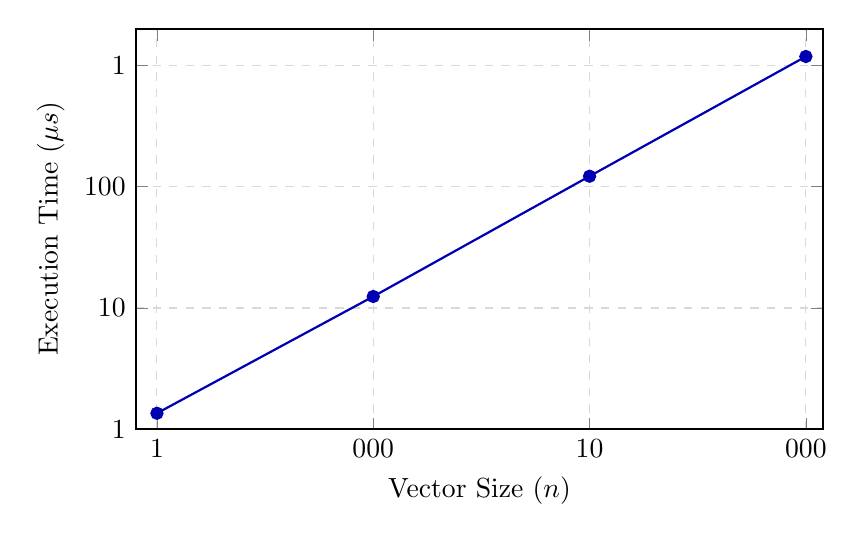
\begin{tikzpicture}
\begin{axis}[
    xlabel={Vector Size ($n$)},
    ylabel={Execution Time ($\mu s$)},
    xmode=log,
    ymode=log,
    log basis x=10,
    log basis y=10,
    xmin=800,
    xmax=1200000,
    ymin=1,
    ymax=2000,
    xtick={1000,10000,100000,1000000},
    xticklabels={1,000,10,000,100,000,1,000,000},
    ytick={1,10,100,1000},
    yticklabels={1,10,100,1,000},
    grid=major,
    grid style={dashed,gray!30},
    width=0.85\columnwidth,
    height=0.55\columnwidth,
    thick
]
\addplot[color=blue!70!black, mark=*, mark size=2pt, thick]
coordinates {(1000,1.357) (10000,12.443) (100000,121.893) (1000000,1181.843)};
\end{axis}
\end{tikzpicture}
\caption{Mean preprocessing execution time vs.\ vector size ($n$), log-log scale evidencing $O(n)$ linear behavior. Means over six input types, CLI tool seed 42.}\label{fig:precost}
\end{figure}

% Tabela 5

\begin{table}[!t]
\caption{Mean symmetric-preprocessing cost vs.\ vector size (mean over six types; CLI tool, seed 42). Point $n{=}20{,}000$ included exclusively for linearity characterization.\label{tab:precost}}%
\begin{tabular*}{\columnwidth}{@{\extracolsep\fill}rrr@{\extracolsep\fill}}
\toprule
Size & Pre ($\mu$s) & ns/element\\
\midrule
1,000 & 1.36 & 1.36\\
5,000 & 6.25 & 1.25\\
10,000 & 12.44 & 1.24\\
20,000 & 24.56 & 1.23\\
100,000 & 121.89 & 1.22\\
1,000,000 & 1,181.84 & 1.18\\
\botrule
\end{tabular*}
\end{table}

\subsection{Total Sorting Time and Per-Algorithm Analysis}
Total-time evaluation reveals a dichotomy: adaptive quadratic algorithms gain wherever absolute inversion reduction $\Delta I$ is large (13.3--99.9+\% at $n{=}10{,}000$), because the modest linear scan ($\approx 1.2$~ns/element) is amortized by suppressed local work. Mechanistically, \emph{Insertion Sort} time per inversion is strikingly regular---$\approx$0.22\,ns/inversion on Random, Turtles, Zigzag, Reversed, and Duplicates at $n{=}10{,}000$ (e.g.\ $5{,}506.86\,\mu s/24{,}960{,}120$)---so its gains track $\Delta I$ directly (Almost Sorted deviates at 0.28\,ns/inversion, consistent with overhead dominance at small $I$). \emph{Bubble Sort} time, by contrast, is nearly flat (16--24\,ms) across inputs whose $I$ spans two orders of magnitude: its pass count follows the maximum left-displacement, not $I$. Hence its modest Random gain ($+13.3\%$ despite $-$45\% inversions) versus collapse to $\approx$1 pass on aligned inputs ($\times$1,084--2,073 speedups). In contrast, $O(n\log n)$ methods respond qualitatively distinctly.

\emph{Merge Sort} shows mixed results by non-overlapping-CI criterion. Gain concentrates in topologies where preprocessing eliminates structural disorder: \emph{Reversed} ($+13.1\%$) and \emph{Zigzag} ($+14.8\%$) at $n=10{,}000$, with increasing gains to $+18.5\%$ at $n=10^6$ (Table~\ref{tab:times1M}). In \emph{Random}, \emph{Turtles}, and \emph{Almost Sorted}, however, the total degrades significantly. Part of these degradations is arithmetic: e.g.\ Merge/Random at $n{=}10{,}000$ slows by $+15.1\,\mu s$ against a mean $C_{\text{pre}}$ of $12.44\,\mu s$, so overhead alone accounts for most of the gap; per-topology $C_{\text{pre}}$ decomposition (same-harness measurement) is pending (Section~3.5).

\emph{Quicksort}, implemented with three-way partitioning and median-of-three, shows systematic degradation under preprocessing. Loss is mild in most topologies ($-3\%$ to $-5\%$ at $n{=}10{,}000$ in \emph{Random}, \emph{Turtles}, \emph{Zigzag}, \emph{Almost Sorted}), but sharp in \emph{Duplicates} ($-31.3\%$) and \emph{Reversed} ($-36.8\%$), always with non-overlapping CIs. Again the overhead scale matters: Quicksort/Duplicates slows by $+14.08\,\mu s$ at $n{=}10{,}000$ (mean $C_{\text{pre}}$ $12.44\,\mu s$) and $+1.31$\,ms at $n{=}10^6$ (mean $C_{\text{pre}}$ $1.18$\,ms), so most of the degradation is the preprocessing cost itself rather than a disturbed key distribution. The \emph{Reversed} case additionally exposes an implementation-specific anomaly: the preprocessed (sorted) vector sorts \emph{slower} (591.80\,ms at $n{=}10^6$) than the random one (55.75\,ms), and scaling from $n{=}10^4$ to $10^6$ is $\approx$884$\times$ on Reversed ($\approx n^{1.45}$) versus $\approx$147$\times$ on Random ($\approx n^{1.08}$). Median-of-three favors sorted inputs in theory, so no median-based explanation is offered; the partitioning behavior on ordered inputs in this implementation requires dedicated validation (comparison counts, reference quicksort), left as future work.\footnote{Times and inversion counts are direct measurements (Tables~\ref{tab:inversions} and~\ref{tab:times}); partitioning and branch-prediction attributions are explanatory hypotheses, not direct measurements (unavailable on Windows, Section~3.5).}

Thus for the $O(n\log n)$ class, the technique is not beneficial in the evaluated implementation, with point exceptions (Merge/Zigzag and Merge/Reversed at both scales; Quicksort/Almost Sorted $+11.1\%$ only at $n{=}10^6$, after $-3.0\%$ at $n{=}10{,}000$ and $-9.3\%$ at $n{=}10^5$). These results delimit preprocessing applicability, indicating inversion reduction alone does not guarantee gains for this class.

\emph{Selection Sort} behavior is consistent with its non-adaptive nature: since comparison count is fixed ($n(n-1)/2$) regardless of initial configuration, inversion reduction yields no systematic gain. Variations span $-1.1\%$ to $+3.3\%$; by the stated non-overlap rule, Random, Almost Sorted, and Duplicates are non-significant (overlapping CIs), while Turtles ($+3.3\%$) and Zigzag ($+1.9\%$) are small but statistically significant deviations, and \emph{Reversed} shows consistent $\approx$12\% degradation at $n=10{,}000$ ($18{,}262.67\pm121.85\,\mu s$ vs.\ $20{,}515.49\pm49.68\,\mu s$; non-overlapping CIs), reproduced at $n=100{,}000$ ($-12.8\%$, $1{,}849.65\pm9.39$~ms vs.\ $2{,}086.10\pm7.92$~ms). Note the framing: the pure Reversed cell (18.26\,ms) is the fast outlier among otherwise 20.5--21.5\,ms cells, so the ``degradation'' is relative to an anomalously fast baseline.

Since preprocessing transforms reversed input into an ordered sequence, minimum search per scan would find the smallest element at the first candidate; expected gain would be merely avoiding one swap per iteration, not justifying observed degradation. One hypothesis involves microarchitectural factors---specifically CPU \emph{branch predictor} behavior \cite{hennessy_computer_2019,edelkamp_blockquicksort_2016}---but both always-taken and never-taken branch patterns are highly predictable, so this hypothesis is weak as stated; assembly inspection (conditional-move vs.\ branch) and per-iteration minimum-update counts are needed to test it. It remains a hypothesis, not a measurement (unavailable on Windows, Section~3.5). Importantly, variation magnitude is limited (at most $\sim$12\%) with no systematic gain---consistent with the prediction that a non-adaptive algorithm does not exploit inversion reduction~\cite{estivill-castro_survey_1992}.

By simultaneously accessing opposite vector ends, symmetric preprocessing introduces additional control dependencies and increases instructions per element. On random instances, internal swap conditions (\texttt{if A[i] > A[j]}) become hard for the branch predictor~\cite{edelkamp_blockquicksort_2016,kaligosi_branch_2006}. Consequently, where inversion reduction is modest, architectural penalties and extra instruction cost outweigh logical-restructuring benefits.

Fig.~\ref{fig:times} synthesizes this dynamic: expressive exploitation in adaptive quadratic methods, mixed \emph{Merge Sort} response, systematic three-way-\emph{Quicksort} degradation, and neutral non-adaptive \emph{Selection Sort} (except Reversed). Table~\ref{tab:times1M} complements analysis for $n{=}10^6$ in quasilinear methods.

% Figura 3

\begin{figure*}[!t]%
\centering
\begin{tikzpicture}
\begin{groupplot}[
    group style={group size=2 by 3, horizontal sep=45pt, vertical sep=65pt},
    ylabel={Time ($\mu s$)},
    width=0.42\textwidth,
    height=4cm,
    ymode=log,
    ymin=1,
    symbolic x coords={Random,Turtles,Zigzag,AlmostSorted,Duplicates,Reversed},
    xtick=data,
    ymajorgrids,
    x tick label style={font=\scriptsize, rotate=35, anchor=north east, inner sep=1pt},
    title style={font=\small\bfseries},
    every axis/.append style={ybar, bar width=3.8pt},
    legend style={at={(1.87,0)}, anchor=north, legend columns=1, font=\footnotesize},
]
\nextgroupplot[title=Insertion Sort]
\addplot[draw=black, fill=black!55] table[x=tipo, y=puro_us] {resultados/fig_tempos_insertion.csv};
\addplot[draw=black, fill=black!20] table[x=tipo, y=com_pre_us] {resultados/fig_tempos_insertion.csv};
\nextgroupplot[title=Bubble Sort]
\addplot[draw=black, fill=black!55] table[x=tipo, y=puro_us] {resultados/fig_tempos_bubble.csv};
\addplot[draw=black, fill=black!20] table[x=tipo, y=com_pre_us] {resultados/fig_tempos_bubble.csv};
\nextgroupplot[title=Selection Sort]
\addplot[draw=black, fill=black!55] table[x=tipo, y=puro_us] {resultados/fig_tempos_selection.csv};
\addplot[draw=black, fill=black!20] table[x=tipo, y=com_pre_us] {resultados/fig_tempos_selection.csv};
\nextgroupplot[title=Merge Sort]
\addplot[draw=black, fill=black!55] table[x=tipo, y=puro_us] {resultados/fig_tempos_merge.csv};
\addplot[draw=black, fill=black!20] table[x=tipo, y=com_pre_us] {resultados/fig_tempos_merge.csv};
\nextgroupplot[title=Quicksort]
\addplot[draw=black, fill=black!55] table[x=tipo, y=puro_us] {resultados/fig_tempos_quick.csv};
\addplot[draw=black, fill=black!20] table[x=tipo, y=com_pre_us] {resultados/fig_tempos_quick.csv};
\legend{Pure, With preprocessing}
\end{groupplot}
\end{tikzpicture}
\caption{Temporal comparison between pure and symmetric-preprocessed sorting ($n=10{,}000$), log scale.}\label{fig:times}
\end{figure*}

% Tabela 6

\begin{table*}[!t]
\caption{Mean time (ms) and preprocessing gain for 1,000,000-element vectors---quasilinear methods only (quadratic omitted for temporal infeasibility). Source: Criterion, 50 samples, 95\% CI.\label{tab:times1M}}%
\begin{tabular*}{\textwidth}{@{\extracolsep\fill}llrrr@{\extracolsep\fill}}
\toprule
Algorithm & Type & Pure (ms) & With pre (ms) & Gain\\
\midrule
Merge Sort & Random & 66.14 $\pm$ 0.75 & 67.12 $\pm$ 0.76 & -1.5\%\\
Merge Sort & Turtles & 17.92 $\pm$ 0.30 & 20.03 $\pm$ 0.51 & -11.8\%\\
Merge Sort & Zigzag & 19.39 $\pm$ 0.39 & 15.81 $\pm$ 0.26 & +18.5\%\\
Merge Sort & Almost Sorted & 20.39 $\pm$ 0.39 & 21.34 $\pm$ 0.39 & -4.7\%\\
Merge Sort & Duplicates & 25.85 $\pm$ 0.42 & 25.09 $\pm$ 0.26 & +2.9\%\\
Merge Sort & Reversed & 18.46 $\pm$ 0.47 & 15.46 $\pm$ 0.19 & +16.2\%\\
Quicksort & Random & 53.83 $\pm$ 0.18 & 55.75 $\pm$ 0.26 & -3.6\%\\
Quicksort & Turtles & 151.34 $\pm$ 0.86 & 157.07 $\pm$ 3.10 & -3.8\%\\
Quicksort & Zigzag & 458.73 $\pm$ 2.59 & 506.44 $\pm$ 3.06 & -10.4\%\\
Quicksort & Almost Sorted & 42.61 $\pm$ 0.27 & 37.88 $\pm$ 0.27 & +11.1\%\\
Quicksort & Duplicates & 4.39 $\pm$ 0.02 & 5.70 $\pm$ 0.03 & -29.9\%\\
Quicksort & Reversed & 416.59 $\pm$ 2.02 & 591.80 $\pm$ 4.62 & -42.1\%\\
\botrule
\end{tabular*}
\end{table*}

Values at $n{=}10^6$ replicate the $n{=}10{,}000$ pattern: Merge Sort gains restricted to Zigzag ($+18.5\%$) and Reversed ($+16.2\%$), systematic Quicksort degradation except Almost Sorted ($+11.1\%$), confirming applicability delimitation to adaptive methods. At $n{=}10^6$ the only overlapping-CI cell is Merge/Random ($-1.5\%$); all other quasilinear cells are significant, including Merge/Duplicates ($+2.9\%$).

Fig.~\ref{fig:gainn} extends the picture across collected sizes ($n{=}1{,}000$--$10^6$, same Criterion means): Insertion/Random gains are stable (34.5--44.2\%), Bubble/Random modest with an uptick at $10^5$ (13.0--25.6\%), Merge/Zigzag and Merge/Reversed grow monotonically (7.5--18.5\% and 4.0--16.2\%), Quicksort/Random stays near $-4$ to $-7\%$, and Quicksort/Almost Sorted is non-monotonic ($-7.6$, $-8.4$, $-3.0$, $-9.3$, $+11.1\%$), flipping sign only at $10^6$---evidence that size trends do not uniformly stabilize and must be reported per topology.

\begin{figure}[!t]
\centering
\begin{tikzpicture}
\begin{axis}[
    xlabel={Vector size $n$ (log scale)},
    ylabel={Gain (\%)},
    xmode=log,
    log basis x=10,
    xmin=800, xmax=1200000,
    ymin=-15, ymax=50,
    xtick={1000,5000,10000,100000,1000000},
    xticklabels={1,000,5,000,10,000,100,000,1,000,000},
    ymajorgrids, xmajorgrids,
    grid style={dashed,gray!30},
    width=0.9\columnwidth, height=5.2cm,
    legend style={at={(0.5,-0.32)}, anchor=north, legend columns=2, font=\scriptsize},
    thick
]
\addplot[color=black, mark=*, mark size=1.6pt, thick] table[x=n, y=insertion_random] {resultados/fig_gain_vs_n.csv};
\addplot[color=black!60, mark=square*, mark size=1.6pt, thick, dashed] table[x=n, y=bubble_random] {resultados/fig_gain_vs_n.csv};
\addplot[color=black, mark=triangle*, mark size=1.8pt, thick, dotted] table[x=n, y=merge_zigzag] {resultados/fig_gain_vs_n.csv};
\addplot[color=black!60, mark=diamond*, mark size=1.8pt, thick, dashdotted] table[x=n, y=merge_inverted] {resultados/fig_gain_vs_n.csv};
\addplot[color=black, mark=x, mark size=2pt, thick] table[x=n, y=quick_random] {resultados/fig_gain_vs_n.csv};
\addplot[color=black!60, mark=+, mark size=2pt, thick, dashed] table[x=n, y=quick_almostsorted] {resultados/fig_gain_vs_n.csv};
\legend{Insertion/Random, Bubble/Random, Merge/Zigzag, Merge/Reversed, Quicksort/Random, Quicksort/AlmostSorted}
\end{axis}
\end{tikzpicture}
\caption{Preprocessing gain vs.\ input size for selected algorithm--topology pairs (same Criterion means as Tables~\ref{tab:times}--\ref{tab:times1M}; quadratic methods capped at $n{=}10^5$).}\label{fig:gainn}
\end{figure}

\section{Conclusion}\label{sec:conclusion}
This work presented and evaluated an $O(n)$ symmetric preprocessing for inversion-count reduction in sorting-algorithm input sequences. On non-aligned inputs it removed 40--62\% of inversions at $\approx$1.2\,ns/element, yielding 13--42\% gains in adaptive quadratic algorithms (Insertion Sort and Bubble Sort) at $n{=}10{,}000$; near-total inversion elimination and $\times$300--2,000 speedups occurred only on symmetry-aligned inputs (Reversed, Zigzag) and must not be generalized. Gains materialize when sorting-cost reduction exceeds preliminary-step cost, satisfying $C_{\text{pre}} + C_{\text{sort}} < C_{\text{original}}$. All comparisons are against the same algorithm without preprocessing; comparison against the fastest available sorter is future work.

For the evaluated non-adaptive quadratic algorithm, Selection Sort showed no systematic gain ($-1.1\%$ to $+3.3\%$, significant only in Turtles, Zigzag, and Reversed under the stated rule), except consistent $\sim$12\% degradation on fully reversed input (non-overlapping 95\% CIs at $n{=}10{,}000$ and $n{=}100{,}000$), hypothesized---not established---to involve microarchitectural effects. This theoretically predicted neutrality via comparison-count invariance ($n(n-1)/2$) delimits that inversion reduction does not convert into gain for non-adaptive methods.

In evaluated $O(n \log n)$ algorithms, the method revealed important limitations. With the used Quicksort implementation (three-way partitioning and median-of-three), preprocessing caused systematic degradation---about $3\%$--$5\%$ at $n{=}10{,}000$ in most topologies ($-10.4\%$ for Zigzag at $n{=}10^6$) and $\approx$30\%--42\% in \emph{Duplicates} and \emph{Reversed} (non-overlapping CIs)---largely on the scale of preprocessing overhead itself, plus an unexplained ordered-input anomaly in this implementation that requires dedicated validation.

In Merge Sort effects were mixed, with gains restricted to topologies most structurally affected by symmetric scanning (Zigzag $+14.8\%$ at $n{=}10{,}000$ and $+18.5\%$ at $n{=}10^6$; Reversed $+13.1\%$ and $+16.2\%$) and degradation elsewhere. Practical viability must therefore be strictly conditioned on adaptive quadratic algorithms, not extending to quasilinear methods generally and particularly not benefiting non-adaptive algorithms like Selection Sort.

As future work, we recommend (i) closed-form theoretical derivation of expected inversion reduction under random input in Hwang et al.'s framework~\cite{hwang_presorting_2000}, including the swap-monotonicity lemma sketched in Section~3.4; (ii) competitive baselines (\texttt{sort\_unstable}, run-detection with $O(n)$ reversal) and non-aligned topologies including small $n$ (16--512) and real data; (iii) same-harness per-topology $C_{\text{pre}}$ decomposition, paired bootstrap inference, multi-seed pools, and Quicksort validation against a reference implementation; (iv) Linux-environment tests with \texttt{perf\_event} infrastructure, enabling direct \emph{cache-miss} and \emph{branch-misprediction} measurement; and (v) alternative partitionings and adaptive techniques such as \emph{BlockQuicksort}~\cite{edelkamp_blockquicksort_2016} and \emph{Timsort}~\cite{auger_timsort_2018} as comparative baselines.

\bibliographystyle{TBench}
\bibliography{reference}
\end{document}
